\documentclass{homework}

\usepackage{graphicx}
\usepackage{xspace}


\newcommand{\kat}{Kathará\xspace}
\newcommand{\opn}{OPNsense\xspace}
\newcommand{\vb}{VirtualBox\xspace}

\newcommand{\client}{\textit{client}\xspace}
\newcommand{\dmz}{\textit{DMZ}\xspace}
\newcommand{\ser}{\textit{internal server}\xspace}
\newcommand{\intfw}{\textit{intfw}\xspace}
\newcommand{\mainfw}{\textit{mainfw}\xspace}

\newcommand{\lan}{\textit{LAN}\xspace}
\newcommand{\opt}{\textit{OPT1}\xspace}
\newcommand{\wan}{\textit{WAN}\xspace}


\title{Practical Network Defense - Lab 6}
\subtitle{LDAP on ACME co.}
\author{Alessandro Serpi - 1647244}
\date{3 May 2019}


\begin{document}
    \maketitle
    \tableofcontents
    
    
    \pagebreak
    \section{Introduction}
    LDAP stands for Lightweight Directory Access Protocol, an open standard for accessing and maintaining directory information services.
    
    In this laboratory, we will use LDAP to perform centralised authentication.
    Username and password of administrative users will be stored into a Zentyal domain controller and the firewalls will perform verification queries at each login attempt.
    
    Zentyal is an open source groupware supporting Samba (among other protocols) based on Ubuntu LTS.
    The assignment was completed in a local environment with the  latest major free release, Zentyal Server Development Edition 6.0.
    
    
    \section{Zentyal configuration}
    \subsection{Network}
    Enable the \textit{Network} module in \textit{Module status} and reboot the server.
    In \textit{System} $\triangleright$ \textit{General}, change the hostname to \texttt{dc} and the domain to \texttt{pndeflab.edu}.
    Then, enable \textit{Network} in \textit{Module status} and reboot the server.
    
    In \textit{Network} $\triangleright$ \textit{Interfaces} configure the internal interface \texttt{eth0} with static address \texttt{100.64.1.2}. 
    Then, in \textit{Network} $\triangleright$ \textit{Gateways}, assign to the gateway on interface \texttt{eth0} (modifying an existing gateway or creating a new one, if necessary) the IP address \texttt{100.64.1.2}.memorise
        
    \subsection{Firewall and DNS}
    Enable \textit{Firewall} and \textit{DNS} modules in \textit{Module status} and reboot the server.
    While the former module is already configured, it is necessary to set up the latter.
    
    In \textit{DNS}, section \textit{Forwarders}, add a known DNS server.
    In section \textit{Domains}, click on the cog wheel in row \texttt{pndeflab.edu} and column \textit{Hostnames}.
    Then, add all relevant hosts in the network, inserting for each one all their local IP addresses.
    
    Open a terminal (either using the virtual machine graphical interface or through an SSH connection) with root privileges and edit the file \texttt{etc/zentyal/dns.conf}, appending \texttt{100.64.0.0/16} to the line starting with \texttt{intnets = }. Then, reboot the server.
    
    \subsection{Remote logging}
    Open a terminal with root privileges and append the line \texttt{*.* @100.64.1.3} to the file \texttt{/etc/rsyslog.d/50-default.conf} and reboot the server.

    \subsection{LDAP}
    Enable the \textit{Domain Controller and File Sharing } module in \textit{Module status} and reboot the server.
    
    In \textit{Users and Computers} $\triangleright$ \textit{Manage}, add a new group \texttt{Firewalls} clicking on the \textit{Groups} folder, then on the green plus sign and completing the form.
    Similarly, add a new \texttt{PND\_Group} group for the administrators.
    
    Add a new computer account for the internal firewall clicking on the \textit{Groups} folder, then on the green plus sign and filling the form as follows (taking care to choose a secure password):
    \begin{figure}[H]
        \centering
        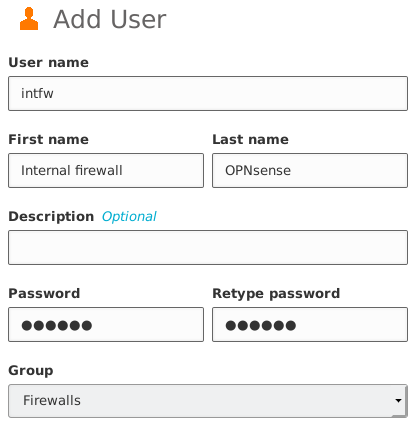
\includegraphics[width=0.7\linewidth]{images/intfw}
        \label{fig:group}
    \end{figure}
    \noindent Then, add another account for the main firewall in the same fashion.
    
    Finally, add a new User account for each admin, inserting them in the \texttt{PND\_Group} group.
    
    
    \section{\opn internal firewall configuration}
    \subsection{Server}
    Create a new authentication server in \textit{System} $\triangleright$ \textit{Access} $\triangleright$ \textit{Server} with the following settings:
    \begin{figure}[H]
        \centering
        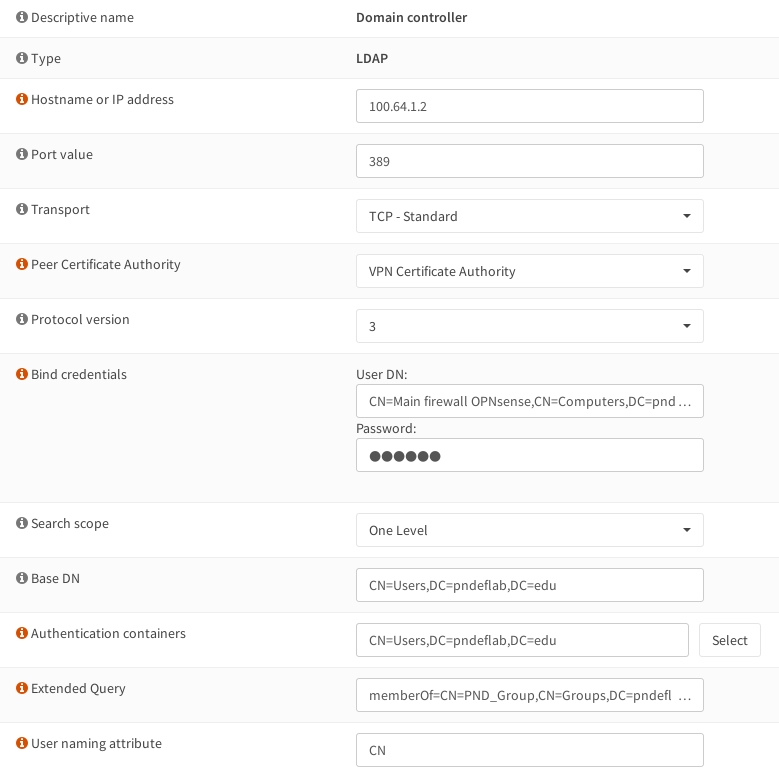
\includegraphics[width=\linewidth]{images/server}
        \label{fig:server}
    \end{figure}
    \vspace{-10pt}

    In field \textit{Bind credentials}, insert the distinguished name and password for the \intfw account created in the domain controller.
    In field \textit{Extended query}, specify that the users must be member of the \texttt{PND\_Group} group.
    After completing the form up to \textit{Base DN}, press the \textit{Select} button adjacent to field \textit{Authentication containers} and choose the only option available.
    
    \subsection{Users}
    In \textit{System} $\triangleright$ \textit{Access} $\triangleright$ \textit{Users}, import start importing new users clicking on the cloud icon.
    Select all showed users and insert them in the \texttt{admin} group.
    
    \subsection{Settings}
    In \textit{System} $\triangleright$ \textit{Settings} $\triangleright$ \textit{Administration}, change the authentication server to \textit{Domain controller}.
    Since superuser access is disabled, it may be advisable to add \texttt{admin} to the list of sudoers.
    \begin{figure}[H]
        \centering
        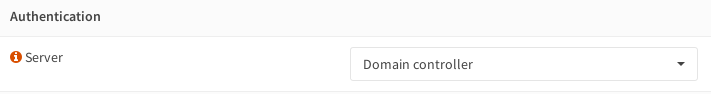
\includegraphics[width=\linewidth]{images/settings}
        \label{fig:settings}
    \end{figure}
    \vspace{-10pt}
    
    If SSH is enabled, add \texttt{admin} to the SSH login groups and disable root login.
    
    
    \section{\opn main firewall configuration}
    Follow the configuration section for the internal firewall, changing the bind account to the one created for \texttt{mainfw}.
    In the internal firewall, create a rule for allowing LDAP traffic from the main firewall to the domain controller.
    \begin{figure}[H]
        \centering
        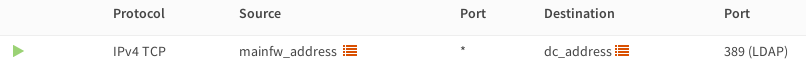
\includegraphics[width=\linewidth]{images/rule}
        \label{fig:rule}
    \end{figure}
    \vspace{-25pt}
    
    
    \section{Test of the configuration}
    Testing was performed manually, trying to login in the two firewalls, both in the web GUI and the physical terminal.
    Using the built-in root user had a negative outcome, while using a LDAP account gave access to both the web GUI and the shell.
    
    
    \section{Final remarks}
    \opn has a lacklustre LDAP support.
    
    The primary shortcoming is the manual user configuration: the usefulness of a central domain controller is greatly diminished if admins must import locally and configure new users in each firewall.
    
    Another deficiency is the non-existent group support.
    A sensible approach would be inserting newly-imported users into local groups with the same names as their LDAP groups (optionally creating those which do not exist) in order to ease privilege assignment; instead, LDAP groups are completely ignored.
    
    Lastly, the documentation is not up to date: some icons are different (e.g. the user import icon) and some settings are located in different sections (e.g. the active authentication servers).
\end{document}
